\documentclass[conference]{IEEEtran}
\IEEEoverridecommandlockouts
\usepackage{cite}
\usepackage{amsmath,amssymb,amsfonts}
\usepackage{algorithmic}
\usepackage{graphicx}
\usepackage{textcomp}
\usepackage{xcolor}
\usepackage{graphicx}
\usepackage{caption}
\usepackage{tabularx}
\def\BibTeX{{\rm B\kern-.05em{\sc i\kern-.025em b}\kern-.08em
    T\kern-.1667em\lower.7ex\hbox{E}\kern-.125emX}}
\begin{document}

\title{Ms. TROMM \\
- A Wise Secretary Always Thinking about You\\
}

\author{\IEEEauthorblockN{JIN HO KIM}
\IEEEauthorblockA{\textit{Dept. Information System} \\
\textit{Hanyang University}\\
Seoul, Korea \\
rlawlsgh1111@naver.com}
\and
\IEEEauthorblockN{EO JIN LEE}
\IEEEauthorblockA{\textit{Dept. Information System } \\
\textit{Hanyang University}\\
Seoul, Korea \\
djwls0317@gmail.com}
\and
\IEEEauthorblockN{GA HEE HAN}
\IEEEauthorblockA{\textit{Dept. Chinese Language and Literature} \\
\textit{Hanyang University}\\
Seoul, Korea \\
sarahan774@gmail.com}
\and
\IEEEauthorblockN{YU JIN HER}
\IEEEauthorblockA{\textit{Dept. Information System } \\
\textit{Hanyang University}\\
Seoul, Korea \\
roqhrcl777@hanyang.ac.kr}
}

\maketitle

\begin{abstract}
Abstract: LG provides LG ThinQ applications to connect its home appliances and consumers and provide consumers with a better experience. The application allows LG's refrigerator, kimchi refrigerator, wash tower, washing machine, dryer, air conditioner, water purifier, styler, air purifier, dishwasher, and oven control with smartphones. Among these many home appliances, we would like to take a deeper look at the link between ‘LG TROMM Styler’ and ‘LG ThinQ’. ‘LG TROMM Styler’ is a home appliance that has been steadily loved by many consumers since its launch because it relieves consumers' discomfort with clothes that are worn every day but cumbersome to manage. LG TROMM Styler provides indoor drying functions, including basic clothing management functions such as steam sterilization, deodorization, and wrinkle relief. This 'LG TROMM Styler' allows you to use functions such as energy monitoring and smartphone remote control when linked to the 'LG ThinQ' application. We would like to propose software that can be used in addition to these applications. This software recommends specific functions of the styler and allows it to operate remotely. Specifically, the software recommends appropriate clothing or styler functions by referring to weather information and calendar information on the user's smartphone. This is expected to help users in their daily lives because it allows users to prepare clothes that meet the weather and schedule in advance.
\end{abstract}

\begin{IEEEkeywords}
Mobile Application, Recommendation System, Artificial Intelligence, Styler, Clothing, Smart Secretary \\ \\
\end{IEEEkeywords}

\begin{table} [h]
    \centering
    \begin{tabular}{l|l|l}
    \hline
    \textit{\textbf{Roles}} & \textit{\textbf{Name}} & \textit{\textbf{Description}}
     & & & \\ \hline
    \textit{\textbf{User/Customer}} & \textit{EO JIN LEE} & \begin{tabular}[c]{@{}l@{}}User/Customer contemplates \\ what functions should be \\ added from the perspective \\ of users or customers. For \\ example, the 'LG TROMM \\ Styler' has a function of adding \\ scent to clothes in addition \\ to simply managing clothes neatly.\\ Consumers also have the need to \\ remotely use these specific \\ functions through the 'LG ThinQ' \\ application. In addition, the \\ application automatically identifies \\ the weather or my schedule and \\ plays a role in considering the \\ needs of the styler's clothing \\ management functions \\ appropriately. \end{tabular} \\ \hline
    
   \end{tabular}
\end{table}

\begin{table} [h]
    \centering
    \begin{tabular}{l|l|l}
    \hline
    \textit{\textbf{\begin{tabular}[c]{@{}l@{}}Product\\ Designer\end{tabular}}} & \textit{YU JIN HER} & \begin{tabular}[c]{@{}l@{}} A product designer is a person \\ with user-centered thinking \\ ability to sympathize with and \\ understand the user's experiences \\ and plays a role in creating \\ an overall framework for product \\ and services. It performs smooth \\ collaboration with other team \\ members with  excellent \\ communication skills. It focuses \\ on the usability of products \\ and services and performs \\ designs to provide better results.\end{tabular} \\ \hline
    \textit{\textbf{\begin{tabular}[c]{@{}l@{}}Software\\ Developer\end{tabular}}} & \textit{GA HEE HAN} & \begin{tabular}[c]{@{}l@{}} A software developer refers to \\ a person who makes software. \\ This includes discovering a \\ meaningful service and accurately \\ grasping the needs of a user who \\ wants to use the service. In \\ addition, there is a need for the \\ ability to design and code \\ these services and user needs \\ in software. Furthermore, the \\ software developer tests the \\ created program.  \end{tabular} \\ \hline
    \textit{\textbf{\begin{tabular}[c]{@{}l@{}}Development\\ Manager\end{tabular}}} & \textit{JIN HO KIM} & \begin{tabular}[c]{@{}l@{}} Development Manager manages \\ the overall part of the project, \\ such as the schedule/planning of \\ the project and the quality of \\ products and services. It also \\ manages/supervises the entire \\ software engineering process of \\ designing, developing, and testing \\ software from accurately grasping \\ user  requirements. In addition, \\ in this process, Development \\ Manager helps project participants \\ communicate smoothly.\end{tabular} \\ \hline
    \end{tabular}
    \renewcommand{\thetable}{\arabic{table}}
    \caption{Roles of Members}
    \label{table}
\end{table}    


\section{Introduction}
\subsection{Overall Introduction}
We are going to create this application with an emphasis on enhancing the value of LG TROMM Styler. Clothing functions as our second skin as one of the three basic elements of life, food, clothing, and shelter. We wear clothes every day and look at what the other person wears. In particular, it constitutes our egos through the process of choosing clothes and the habit of wearing clothes. Clothing is not only a basic purpose of protecting the body, but also a means of representing the value and status of the person wearing the clothes. Likewise, clothes are tools to complete humans, which are social animals.

However, it takes a lot of time and effort to manage the clothes to wear every day. Especially, in Korea, difficulties in managing clothing at home have increased due to air pollution such as fine dust. Due to this situation, the demand for clothing management devices at home increased, and in May 2011, LG launched the ‘LG TROMM Styler’ (hereinafter referred to as ‘Styler’). Styler is loved by allowing clothes to be managed at home for dry cleaning and shows high growth in sales rates. Furthermore, stylers are developing into comprehensive home appliances including indoor dehumidification functions as well as clothing management. 

In addition to this, LG increased device accessibility by linking its app called 'LG ThinQ' with a styler.‘ LG ThinQ’ is a representative home appliance management app that provides smart home services based on AI. With this application, you can control not only home appliances, but also all parts of the house, as well as check product status and malfunctions anytime, anywhere. In a situation in which the market environment is rapidly changing from 'supplier-centered' to 'consumer-centered, LG is providing these services, believing that the role of AI technology has grown.

However, we found that most users always worry in front of the Styler, "What should I wear tomorrow?" This is because they put clothes in the Styler to take full care of them for tomorrow schedule. In this situation, we have introduced an AI-based recommendation system(hereinafter referred to as ‘Ms.TROMM’) to Styler to reduce this time of concern and promote consumer-centered value. 

Ms.TROMM recommends modes that can be operated by the Styler, styling, and scent. First,  Ms.TROMM makes recommendations based on the user's calendar. By linking the calendar, Styler mode is recommended according to the user's schedule, and user can select the Styler operation by their preference. Second, Ms.TROMM uses the weather API to recommend suitable for the weather or a Styler mode that suits with weather. Third, Ms.TROMM identifies the clothes and the material of the clothes in the Styler and recommends the appropriate Styler mode and styling information for the clothes. Finally, data is accumulated through the process of receiving user feedback after all recommendations, and Ms.TROMM provides more sophisticated personalized recommendations. Through this, people can reduce their time of concern in front of the styler every evening or morning, and the need for a styler in our lives will also increase. Also, it is expected that users will be able to receive positive values for LG and styler if Ms.TROMM is installed in the ‘LG ThinQ’ application. We plan to create this application with an emphasis on increasing the satisfaction of styler users through Ms.TROMM, a system that allows users to use stylers and experience better.
\subsection{Problem Statement}\label{SCM}
\begin{itemize}
\item There is an application called ‘LG ThinQ’ as a mobile application that can be used in conjunction with LG home appliances. We thought that it would be better if a recommendation function was included in this application
\item It is very useful to use a styler to manage clothes, but since it takes a lot of time to manage clothes, there is a time constraint to take care of clothes to wear right away in the morning.
\item Therefore, we thought that the styler could be used more effectively if there was software that knew the user’s schedule and weather and sent a message to manage clothes in advance.
\item The software recommends clothes that users will like in the future based on feedback on past users’ tastes and recommendations. In other words, it helps you to use the styler efficiently by controlling the past and the future at once.\\
\end{itemize}

\section{REQUIREMENT}

\subsection{Recommend appropriate styler functions for clothes that are alreaady in the styler.}
Ms.TROMM can identify clothes currently in the styler and recommend appropriate styler functions through interworking with the LG styler. The user can deliver the functions of the styler recommended through Ms.TROMM to the LG styler and request the LG styler for functions suitable for the material of the clothes in the styler. In addition, if the user learns clothes that are frequently used or preferred by the styler, and accordingly, the styler can suggest styling with these clothes or request the styler function according to the user’s usual styler usage pattern.\\


\subsection{Recommend clothes sutable for the situation in conjunction with the user’s calendar and weather information.}
First of all, Ms.TROMM recommends styling suitable for each situation for each activity such as meeting or hobby in conjunction with the user's calendar. For example, suits are recommended on days when meetings are scheduled. In addition, if you are scheduled for a picnic with your family on the weekend, you can recommend a combination of clothes for users and remind them of the schedule. Ms.TROMM can learn words related to the schedule and provide contextual recommendations even if the user writes down difficult or unfamiliar words on the calendar. In addition, after the recommendation, the user may be asked if the recommendation was appropriate and through the feedback process, the user may be provided with a better recommendation provided by Ms.TROMM.
Next, Ms.TROMM may propose styling according to weather information in conjunction with the weather API. In addition, if it is linked to LG's smart mirror, users' clothes can be registered in advance and registered clothes can be used. For example, on days when the daily temperature difference is expected to be large, thick knitwear among registered user's clothes is recommended, and styling is suggested accordingly. In addition, suits can be recommended on days when meetings are scheduled. In addition, if you are scheduled for a picnic with your family on the weekend, you can recommend relatively casual clothes among registered clothes using weather data. After the recommendation, the user may be asked if the recommendation was appropriate and through the feedback process, the user may be provided with a better experience to Ms.TROMM.\\


\subsection{Interworking with the user’s calendar and weather information to recommend scents suitable for the situation and the fragrance system of the styler.}
First of all, Ms.TROMM recommends a scent suitable for each situation in conjunction with the user's calendar, and if the user wants, the recommended scent can be applied to the clothes in the styler. For example, if it is determined to be a holiday through the user's calendar, Ms.TROMM recommends a warm soap scent that allows the user to spend the day comfortably. If the user likes the recommended scent from Ms.TROMM, the user requests the linked LG Styler for the desired scent, and according to the user's request, the LG Styler adds a scent that suits the situation.
Next, since Ms.TROMM utilizes the weather API or learns the situation, users can get recommendations for scents suitable for the situation recommended by Ms.TROMM, and can coat the recommended scents with clothes they want in conjunction with the scent system of the LG Styler. Users will feel more satisfied if recommendations can be made according to the advice of experts related to aroma in this process. For example, if it is predicted to rain through the weather API, "Today is a rainy day. On rainy days, I recommend the warm soap scent recommended by expert A. Do you want me to add scent to the clothes inside the styler? You can recommend it like that, and if the user agrees, "I put on a warm soap scent! It provides reactions such as "Have a good day" and adds scent to clothes through the linked LG Styler's fragrance system. Finally, the recommendation of Ms.TROMM can be more sophisticated whenever the recommendation process proceeds through feedback processes such as "Was today's recommendation accurate?"\\


\subsection{In conjunction with the user’s calendar and weather information, it is recommended to manage clothes suitable for the schedule and weather scheduled in a few days in advance in order to prepare appropriate clothes in advance.}
Since it takes a considerable amount of time to operate the styler’s clothing management function, in reality, operating the styler in the morning when you need to wear clothes immediately to manage your clothes is subject to many restrictions. So, Ms.TROMM recommends that appropriate clothes be kept in the styler and managed by referring to the planned schedule and weather forecast (about three days in advance). For example, if there is a meeting in three days, Ms.TROMM said, “We have a meeting in 3 days, so put your suit in the styler and take care of it in advance. It sends messages such as ~” to help users prepare clothes in advance\\


\subsection{Recommend that you take care of the clothes that have been in the styler.}
Ms.TROMM prioritizes management by scoring the clothes stored in the smart mirror on the basis of “the last day of putting them in the styler, the last day of wearing them, and the last day of disinfection.” And users receive clothing management messages according to these priorities. For example, Ms.TROMM told the user, “I haven’t put OOO clothes in the styler for 2 weeks. Are you still wearing it? I recommend disinfecting clothes” and “The OOO coat has not been in the styler for more than three days, but do you forget it?” And through the Ms.TROMM application, The priority score is displayed as a percentage so that the clothes that are most likely to need the management of the styler can be identified.\\


\subsection{Learn the home environment such as humidity and recommend appropriate functions such as dehumidification depending on the situation.}
Currently, LG Styler users can use a dehumidification function or the like through the Styler. Ms.TROMM can use this function to measure the environment (ex. Humidity, temperature, etc.) of the space where the styler is located and recommend functions (ex. Dehumidification functions, etc.) suitable for the environment through the user’s smart device, which allows users to easily control the styler.\\\\

\section{DEVELOPMENT ENVIRONMENT }
\subsection{Choice of software development platform}
Our main development environment is Windows and MacOS. In the case of Windows, terminals that can be used even in windows such as Powershell were used to create a linux environment, and in the case of MacOS, built-in linux environment and terminals were used. Ms.TROMM in order for consumers to receive recommendations faster and immediately control devices such as stylers and smart mirror. Ms.TROMM was manufactured based on mobile applications. In addition, Ms.TROMM so that more users can use it in various mobile operating systems. The frontend framework of Ms.TROMM selected 'Flutter', a representative cross-platform framework. Currently, Google's Android accounts for the majority of global mobile platforms, and Apple's iPhone accounts for about 15\%, but Apple's iPhone users' consumption patterns and loyalty to electronics are quite different from Android users, and iPad, which accounts for a large portion of the tablet market, so the actual usage rate is very high. In fact, looking at the mobile operating system market share, including the tablet market, it can be seen that the proportion of iOS (including iPadOS) has increased by about 30\%. Therefore, we have adopted Flutter, a mobile/web/desktop cross-platform framework launched by Google based on the Dart Programming language, as a frontend framework, satisfying all of these demands and further considering future desktop applications. In the case of backend server, Python-based Flask, which implements artificial intelligence-based services and has well-established statistical and analysis packages, was adopted. Flask has the advantage of being easy to create API servers and very light. In addition, since Flask has a high degree of freedom, such as being able to change and respond immediately according to the purpose of development when there is not much time left, It was adopted because it was considered the most suitable web framework for Ms.TROMM development.\\ \\

\begin{figure}[]
\centerline{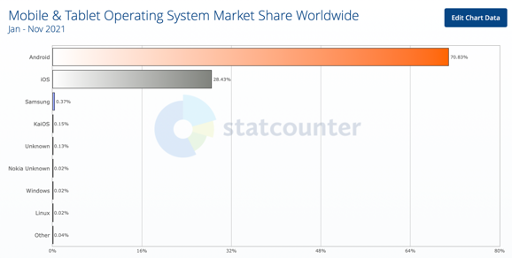
\includegraphics{그림1.png}}
\caption{Mobile \& Tablet OS Market Share Rate}
\label{fig}
\end{figure}

\begin{figure}[]
\centerline{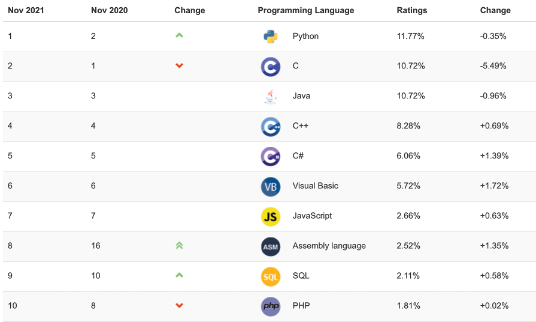
\includegraphics{그림12png.png}}
\caption{TIOBE INDEX}
\label{fig}
\end{figure}


\begin{table}[ht]
    \centering
    \begin{tabularx}{\columnwidth}{X|X}
    \hline
    \textit{\textbf{Name}} & \textit{\textbf{Development Environment}}
     & & \\ \hline
    \textit{\textbf{JIN HO KIM}} & MacOS, Python 3.8.5    
     & & \\ \hline
    \textit{\textbf{EO JIN LEE}} & Windows, Python 3.9.0
     & & \\ \hline
    \textit{\textbf{GA HEE HAN}} & Windows, Python 3.9.2
     & & \\ \hline
    \textit{\textbf{YU JIN HER}} & Windows, Python 3.7.1
     & & \\ \hline
    \end{tabularx}
    \renewcommand{\thetable}{\arabic{table}}
    \caption{Develop Environment}
    \label{tab:table}
\end{table}

\begin{table}[h]
    \centering
    \begin{tabular}{c|l}
    \hline
    \multicolumn{1}{l|}{\textit{\textbf{Tools and Language}}} & \textit{\textbf{Reason}} 
     & & \\ \hline
    \textit{\textbf{Python}} & \begin{tabular}[c]{@{}l@{}} Python is one of the programming languages \\ that many people love around the world. \\ TIOBE announces the rankings of world-\\famous programming languages every month,\\ representing them as "TIOBE INDEX,"\\ and Python was ranked No. 1 programming \\ language loved by people around the world as \\ of November 2021. Python is also the base \\ language for Flask, a web server framework, \\ but it provides excellent modules related \\ to artificial intelligence. In addition, it provides \\ a Pandas, Numpy module, etc. necessary for \\ data analysis and processing of collected data. \end{tabular} \\ \hline
    \textit{\textbf{MySQL}} & \begin{tabular}[c]{@{}l@{}} We need a database that stores data from users \\ who signed up for membership to use the \\ Ms.TROMM service, stores schedule data \\ used for recommendations, and responses from \\ users, and provides better service \\ recommendations based on this. Therefore, \\ we intend to manage the basic database \\ using MySQL. \end{tabular} \\ \hline
    \textit{\textbf{Flutter(Dart)}} & \begin{tabular}[c]{@{}l@{}} Flutter is a Dart language-based cross-platform \\ framework launched by Google. So, \\ Ms.TROMM was developed based on Flutter \\ so that it could be expanded to web and \\ desktop apps in the future. In addition, \\ even though it is a cross-platform, it provides \\ native-class performance and various extensions, \\ makes it easy to check the UI in a simple \\ virtual environment, and supports plug-ins \\ from famous IDE and code editors, so Flutter \\ was selected as the frontend framework. \end{tabular} \\ \hline
    \end{tabular}
    \renewcommand{\thetable}{\arabic{table}}
    \captionsetup{justification=centering}
    \caption{Tools and Programming Languages \\ used for development}
    \label{tab:table}
\end{table}


\begin{figure}[htbp]
\centerline{
\includegraphics{flutter.png}}
\caption{Cross-platfrom framework 'Flutter'}
\label{fig}
\end{figure}


\subsection{Software in use}
\begin{enumerate}
    \item LG ThinQ, LG SmartHome Application\\
    \centerline{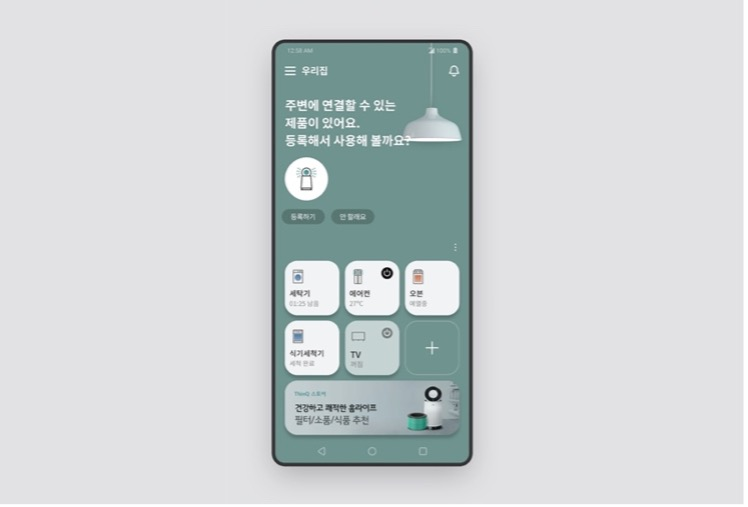
\includegraphics[scale=0.30]{thinkq.jpg}}

        LG Electronics uses the 'LG ThinQ', an application to control its smart home appliances. In addition, in the case of smart mirror, it can be controlled through the 'LG Smart Home' as a key home appliance for the smart home ecosystem that will be built as soon as possible. Through these two apps, LG Electronics will bridge users and smart devices so that users can monitor and control their homes anytime, anywhere. Our application is also an app to build a better ecosystem between users and smart devices. Our app is a smart assistant-like application that integrates the environment in which users use smart devices, checks minor things in advance that users may miss, and recommends the best way. \\ \\
    \\ 
    \item VSCode(Visual Studio Code) \\ \\
\centerline{
\includegraphics{vs.png}}
VSCode is an open source-based text editor published by Microsoft. VSCode is a text editor, not an IDE, but has the advantage of being able to install various expansion packs. In addition, it has its own terminal function. Supporting various languages, The development environment for data and artificial intelligence technologies used by Ms.TROMM is excellent. In addition, VSCode was adopted as a text editor because of its excellent interworking with Git, a version control system.\\ \\ \\ \\ \\ \\ \\ \\ \\ \\ \\ \\ \\ \\
    \item Android Studio \\ 
\centerline{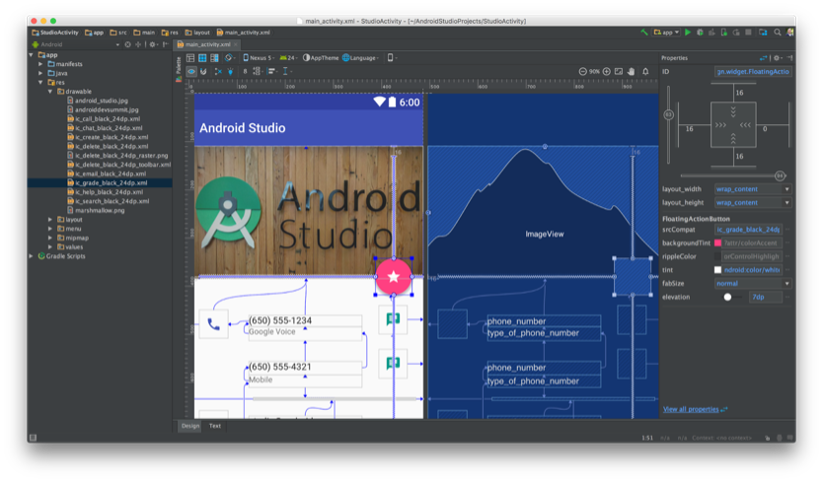
\includegraphics{as.png}}
    In the case of Ms.TROMM, since it is basically a mobile app, an integrated development environment (IDE) for mobile apps was needed, and Android Studio, which team members were relatively familiar with, was adopted as IDE. Both Flutter and Android Studio, which we adopted as the Frontend Framework, are platforms announced by Google, so they are highly interconnected, so there was no big problem in developing them. The advantage of being able to develop while checking the progress of the app through the UI is also the reason for adopting Android Studio. \\ \\
    \item Swagger \\ 
\centerline{
\includegraphics{Swagger.png}}
    Swagger is a framework for Open API Specification (OAS). Swagger is used together with a set of open-source software tools to design, build, document, and use RESTful web services. Swagger includes automated documentation, code generation (into many programming languages), and test-case generation. Simply put, Swagger is an API Spec document. The method of managing APIs through Excel or guide documents requires periodic updates, so it is not easy to manage and takes a long time. So, we can easily manage and test API documents by automating API Spec documents using Swagger. \\ \\    
    \item DBdiagram \\ \\
\centerline{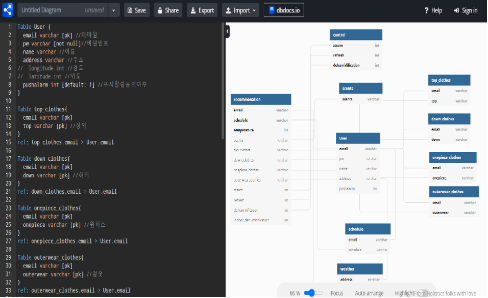
\includegraphics[scale=0.9]{DB.png}}
\\ It is a free, simple tool to draw ER diagrams by just writing code. So, the user can draw entity-relationship diagrams, painlessly. ERD is a very important development product because it can be used to see the model at a glance when implementing functions. Using this site, ERD can be configured through a code similar to SQL. If related codes such as tables and indexes are inserted without drawing ERD separately, ERD is automatically generated. It is also very useful because it can be modified based on code even when modifying.\\ \\ \\ \\
    \item MySQL \\ \\
\centerline{
\includegraphics[scale=0.1]{MySQL.png}}
\\ MySQL is the most widely used open-source database worldwide. It is an open-source relational database management system (RDBMS) that uses the standard database query language SQL (Structured Query Language) and features very fast, flexible, and easy to use. It supports multi-user, multi-threads, and provides an application interface (API) for C, C++, Eiffel, Java, Pearl, PHP, Python scripts, and the like. It can be used in Unix, Linux, and Windows operating systems. The Linux operating system, Apache server program, MySQL, and PHP script language composition are free programs that are developed as open-source despite good interworking, so MySQL was also adopted in the development of Ms. TROMM.\\ \\ \\ \\
    \item SQLAlchemy \\ \\
\centerline{
\includegraphics[scale=0.1]{sqlalchemy.jpg}}
\\ SQLAlchemy is an open-source SQL toolkit and object-relational mapper (ORM) for the Python programming language. The advantage is that it is possible to focus on business logic with object-oriented code. It also increases reuse and maintenance convenience and reduces dependence on DBMS. Because of these advantages, we decided to use SQLAlchemy with Ms. TROMM's recommendation system.\\ \\ \\ \\
    \item SQLite \\ \\
\centerline{
\includegraphics[scale=0.1]{SQLite.png}}
\\ SQLite is a file-based embedded SQL database engine with database management systems such as MySQL and PostgreSQL. It is basically included in Android, iOS, and macOS. It is one of the lightweight DBs mainly used in applications and is a fast, easy-to-use, and free library. Unlike other SQL databases, it does not have a separate server, reads and writes regular disk files directly, and has multiple tables, indexes, triggers, views, etc. in only one file.\\ \\ \\ \\
    \item Adobe XD \\ \\
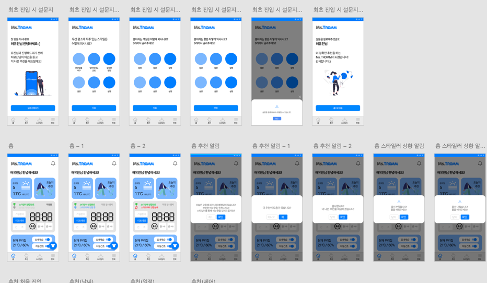
\includegraphics[scale=0.9]{XD.png}
Adobe XD is an application for prototyping PCs, mobile Internet pages, and mobile apps released by Adobe. Since Ms.TROMM is a mobile app-based service, it was necessary to think about how users could feel the best experience when providing the app. Therefore, it is possible to intuitively prototype the operation of an Internet page or app operating in a corresponding environment through Adobe XD. In addition, the app development can be made easier by linking the prototype made in this way with Zeplin.\\ \\ \\
    \item Zeplin\\ \\
    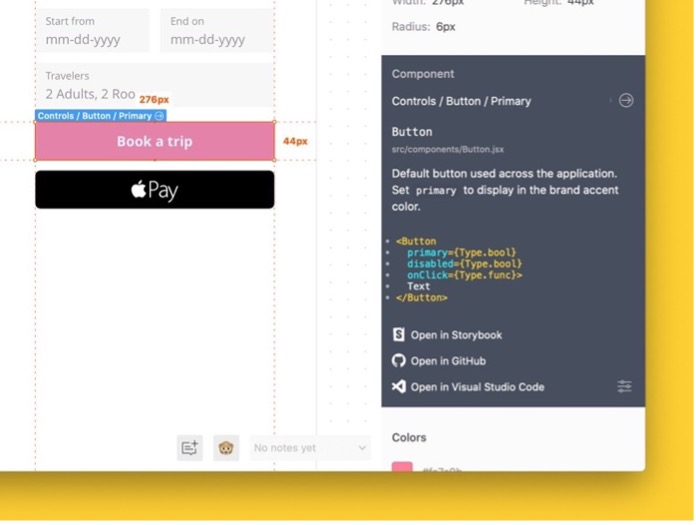
\includegraphics[scale=0.32]{Zp.jpg}
    Zeplin is a software that helps designers and developers collaborate, and through Zeplin, you can convert design elements into development information (e.g., font, size, size, etc.). While developing apps through Zeplin, you can solve problems that may not be faithful to functional implementation while calculating design elements too deeply. \\ \\ \\ \\ \\ \\ \\
    \item Heroku\\\\
    
\includegraphics{Heroku.png}
 \\ \\ Heroku is a service that allows free hosting of websites through git. It is a cloud platform as a service (PaaS) that supports multiple programming languages. In general, when developing or implementing an app, it provides a platform that enables applications to be developed, executed, and managed without the complexity of creating and maintaining related infrastructure. \\
    \item GitHub\\\\
    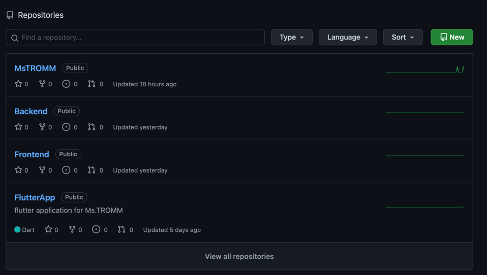
\includegraphics[scale=0.9]{Gtib.png}
 \\ \\ GitHub serves as a repository for Git, a distributed version control system. During development, several people go through a collaborative process of adding and deleting various functions, which can lead to confusion in this process without a version control system. Github is a web-based service that allows you to intuitively understand the team members' version control process. In addition, simple processes such as simply uploading and downloading files can be easily controlled using GUI tools such as Github Desktop. \\
\end{enumerate}{}

\subsection{Task distribution(To be Cont..)}  \\ \\


\section{SPECIFICATION}
    \begin{figure}[htbp]
\centerline{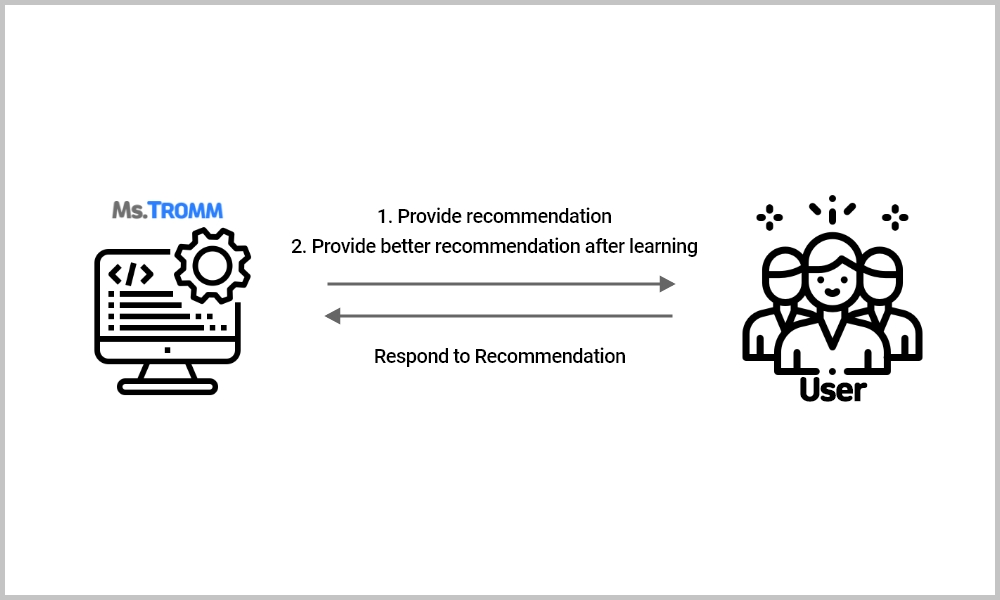
\includegraphics[scale=0.2]{Whole application.jpg}}
\label{fig}
\end{figure}
This picture shows our whole application. Ms. TROMM's recommendation system provides recommendations to users. At this time, the user's reaction is recorded in the DB, and the recommendation system proceeds with learning based on this reaction. And when the next recommendation situation comes, the recommendation system provides recommendations to users again. \\ \\ \\ \\ 

\subsection {Entry} \\
\begin{enumerate}
    \item Splash screen \\ \\
     \centerline{
\includegraphics[scale=0.32]{스플래쉬 화면.jpg}}
    \begin{itemize}
    \item[] This is the start page when you run the app. It is exposed for 1 to 2 seconds not to show an empty page during the app's data loading time. \\ \\ \\ \\
    \end{itemize}
    \item Onboarding screen \\ \\
    \centerline{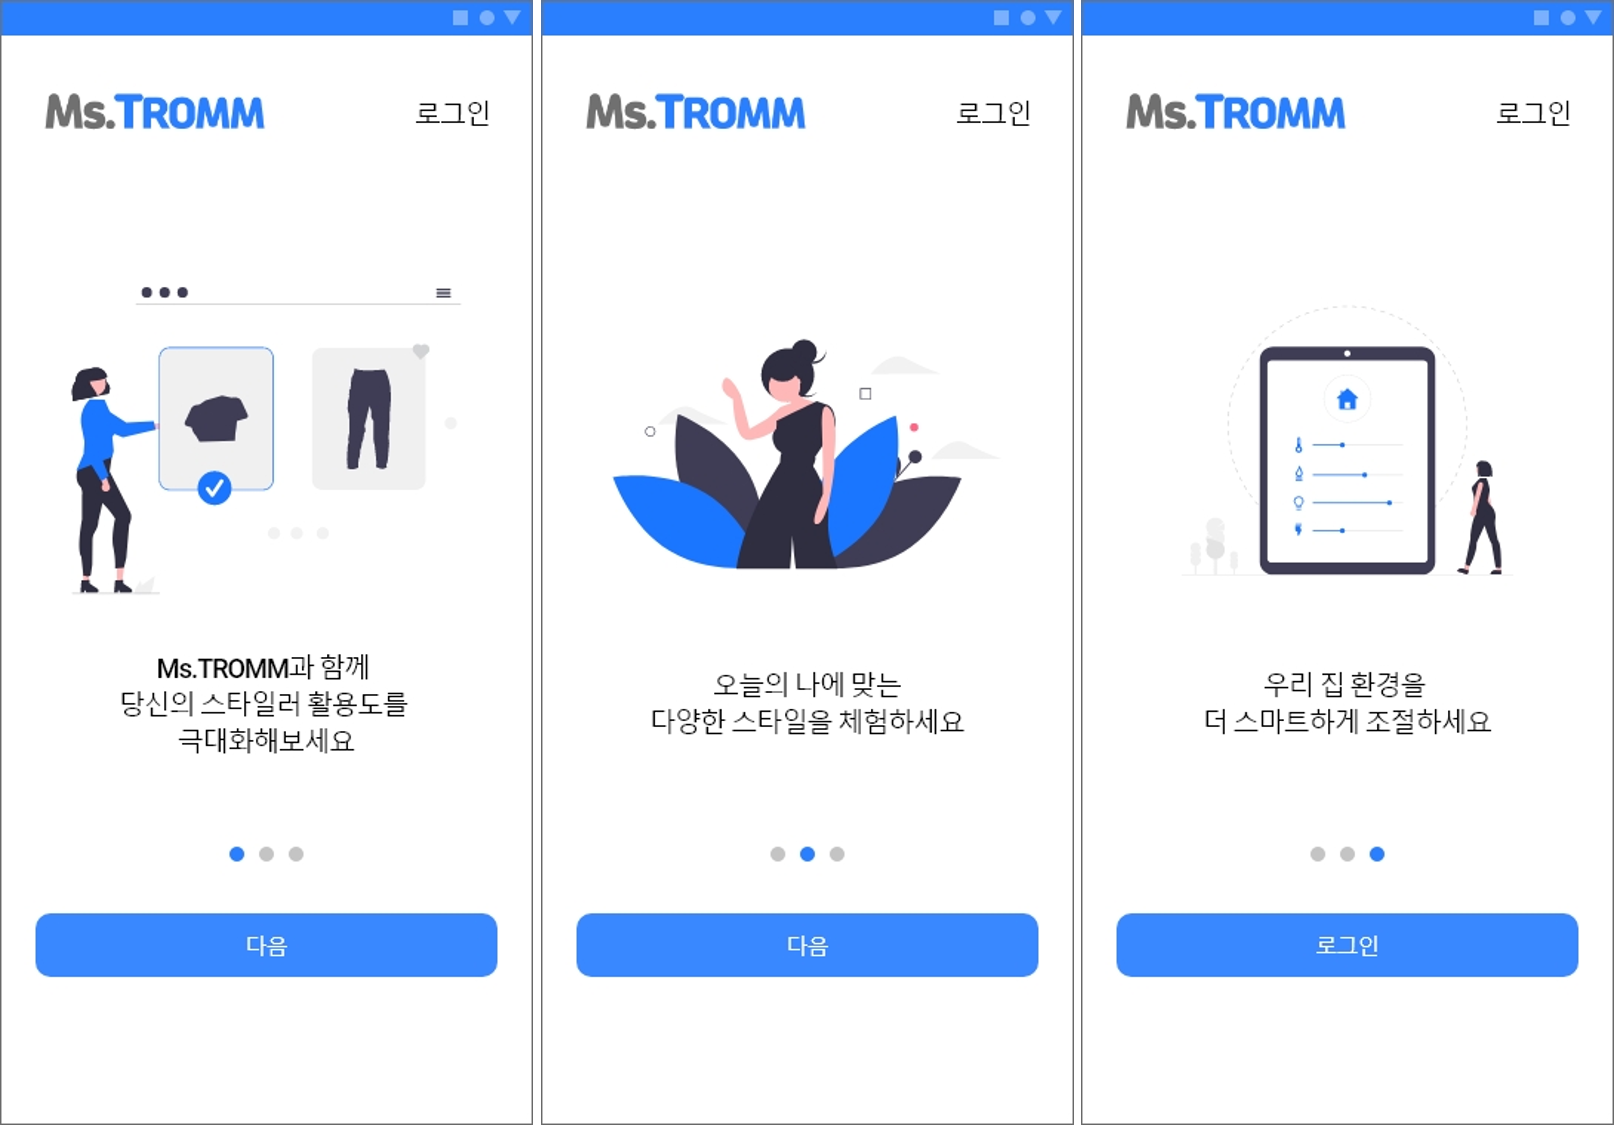
\includegraphics[scale=0.32]{온보딩.png}}
    \begin{itemize}
    \item[] It is a page that prevents the deletion of apps by clearly showing users the reason for the existence of apps. It consists of a total of three pages explaining why Ms.TROMM's main functions and functions are useful.\\ \\ \\
    \end{itemize}
    \item Onboarding Button \\ \\
    {
\includegraphics[scale=0.75]{온보딩_다음.jpg}}
    \begin{itemize}
    \item[] Put the next button at the bottom of the page so that you can move on to the next page.
    \end{itemize}
    {
\includegraphics[scale=0.75]{온보딩_로그인.jpg}}
    \begin{itemize}
    \item[] And on the third page, it changes to the login button to the next button location as shown in the picture. 
    \\ If you have login data on your phone, do not expose the onboarding page. When the splash screen is terminated, the login page is immediately exposed.
    \end{itemize}
    \end{enumerate}
    \break

\subsection {Login} 
Ms.TROMM receives two types of information (email, password) for login.\\
\begin{enumerate}
    \item Login form screen \\ \\
    \centerline{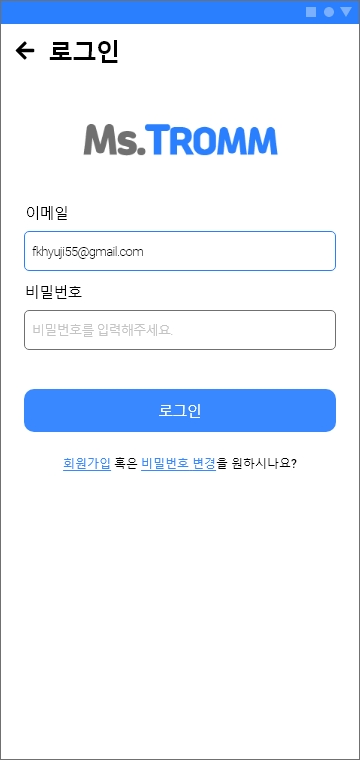
\includegraphics[scale=0.32]{로그인1.jpg}}
    \begin{itemize}
    \item[] A login form screen appears where you can enter your email and password. The login button is exposed at the bottom of the field, and there are buttons below the button to sign up for membership and go to the password change page. \\
    \end{itemize}
    \item Login failed screen \\\\
    \centerline{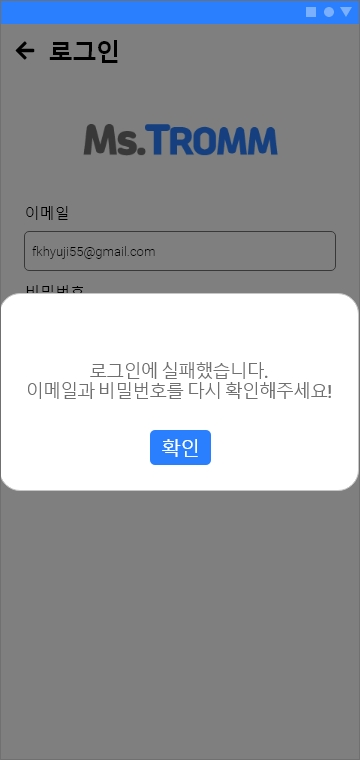
\includegraphics[scale=0.32]{로그인2.jpg}}
    \begin{itemize}
    \item[] If login information that is not in the DB is entered, login failed and a pop-up with 'Please check your email and password again!' comment is displayed at the bottom. When you click the gray area or 'x button' or 'OK button', the pop-up will end and the previous one will be exposed again. \\ \\
    \end{itemize}
    \item Changing the password \\ \\ \\
    \centerline{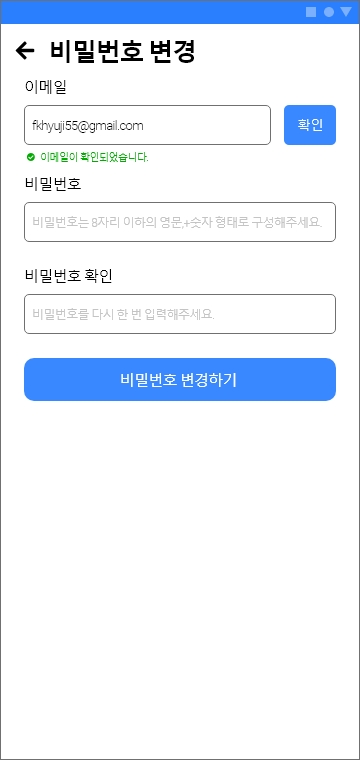
\includegraphics[scale=0.32]{비밀번호 변경.jpg}}
    \begin{itemize}
    \item[] It is a page that supports password change when a user forgets his or her password. In the case of e-mail input, there is an e-mail confirmation field to verify that it is currently in DB. Hereinafter, there is a field where a new password can be set, and there is a password confirmation field to prevent password errors. \\ \\ \\ \\ \\ \\ \\ \\ \\ \\ \\ \\ \\ \\
    \end{itemize}
    \end{enumerate}{}
    
\subsection{Sign up}
This is the membership form page. Ms.TROMM receives three types of information (name, e-mail, password) when signing up for membership. We plan to add documents and personal information utilization tabs that say this information is only used within Ms.TROMM. \\ \\ 

\begin{enumerate} 
    \item Sign up form screen \\ \\ \\
    \centerline{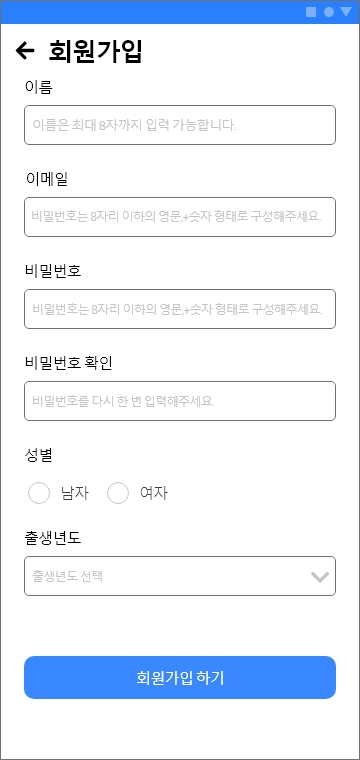
\includegraphics[scale=0.32]{회원가입1.jpg}} \\
    \item[] It consists of fields that receive the name, email, password, and password check. \\
    \begin{itemize}
    \item[-] The name must be entered in 8 characters or less, and we notify you in advance that the name is a necessary element to be called within the app. \\ \\
    \item[-] The e-mail will be exposed to the phrase asking you to follow the e-mail format and enter it.
    \\ \\
    \item[-] The password will be exposed in a combination of English and numbers of less than 8 digits.
    \\ \\
    \item[-] In the case of password verification, the same phrase as the password entered above will be exposed.
    \\
    \item[-] If an input value that does not match the rules is entered in the field, the field is processed red, and a warning statement is exposed at the bottom.
    
          \begin{enumerate} 
          \item Phrases when invalid \\ \\
            \centerline{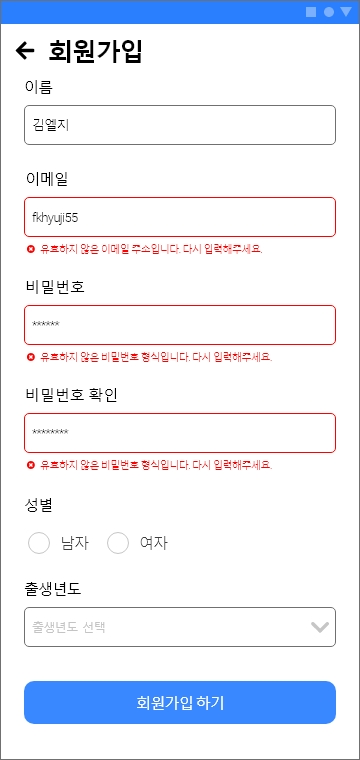
\includegraphics[scale=0.28]{회원가입3.jpg}}
          \begin{enumerate}
          \item The name is not valid. Please input it again.
          \item This is an invalid email format. Please input it again.
          \item This is an invalid password format. Please input it again.
          \item The password does not match. Please input it again.
        \end{enumerate}
    \item[-] \\ If an input value that matches the rule is entered, the field is processed in green, and the phrase "valid value" is exposed at the bottom. \\
    \item Phrases when valid \\ \\ \\
    \centerline{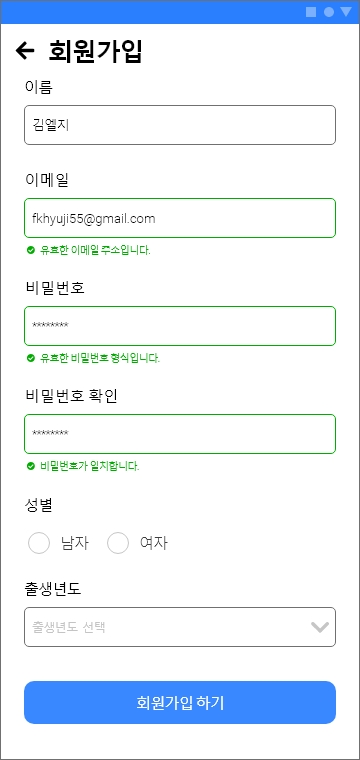
\includegraphics[scale=0.28]{회원가입2.jpg}}
    \begin{enumerate}
\item This is a valid name.
\item This is a valid email format.
\item This is a valid password format.
\item The password matches.
    \end{enumerate}
        \end{enumerate}
          \end{itemize}
    \item Pop-up \\\\
    \centerline{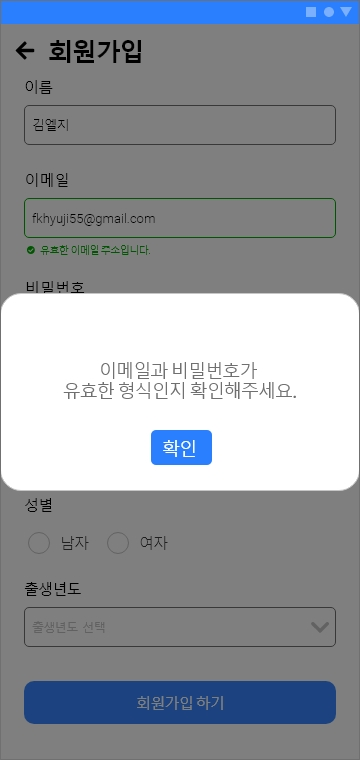
\includegraphics[scale=0.32]{회원가입4.jpg}}
    \begin{itemize}
        \item[] \\ \\ If you click the Sign-up button before the form is not completed, a pop-up with ’All values have not been entered. Please complete the input.' comment is displayed at the bottom. When you click the gray area or 'x button' or 'OK button', the pop-up will end and the previous one will be exposed again.\\ 
    \end{itemize}
    \item Completed page \\ \\
    \centerline{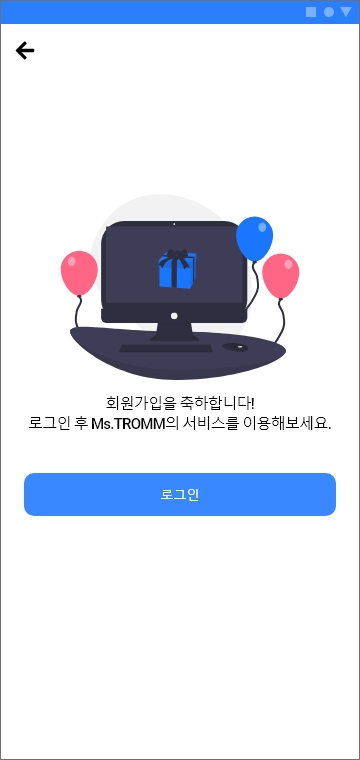
\includegraphics[scale=0.32]{회원가입5.jpg}}
        \begin{itemize}
        \item[] This page is exposed when membership is completed. Click the login button to go to the login screen.
    \end{itemize}
    \end{enumerate}

\subsection{Main Page}
\begin{itemize}
    \item[] When the login is completed, the main page is exposed. When a user with no login record logs in for the first time, the questionnaire page is exposed instead of the main page.
    \item[] At home, you can check four items: notification, today's weather, today's recommendation, basic styler control, and our house status. Also, there is a connection button with a styler or smart mirror, so it is possible to easily check and connect the connection status.\\  
\end{itemize}
\begin{enumerate}
    \item Survey(first time to entry) 
    \begin{enumerate}
    \item Information page \\ \\ \\
    \centerline{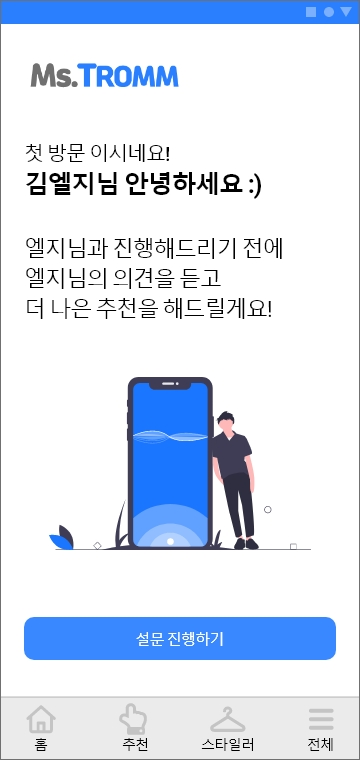
\includegraphics[scale=0.32]{설문지1.jpg}}
    \begin{itemize}
        \item[] \\ \\ This is a page that guides the survey. The survey progress button is exposed at the bottom. The survey consists of contents that will be conducted because it is helpful for the recommendation. \\ \\ \\ \\ \\ \\ \\ \\ \\ \\ \\ \\ \\ \\ \\ \\ \\ \\

    \end{itemize} 
        \item Survey page \\ \\ \\
        \leftline{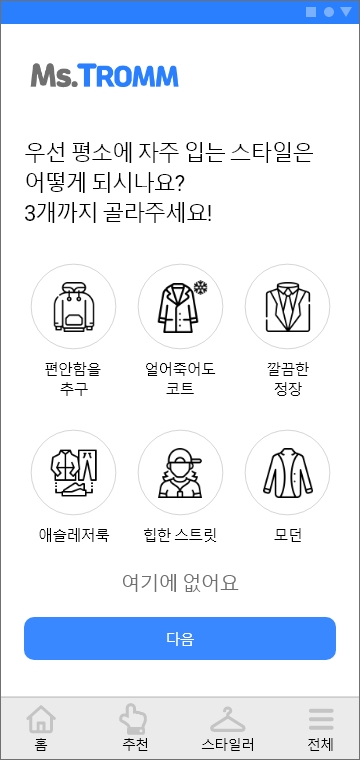
\includegraphics[scale=0.15]{설문지2.jpg}
                   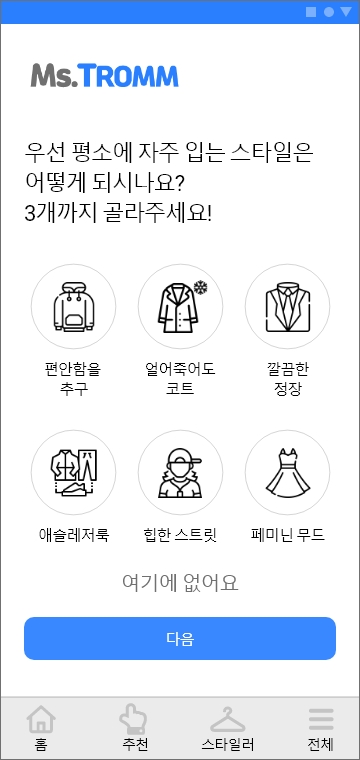
\includegraphics[scale=0.15]{설문지3.jpg}
                   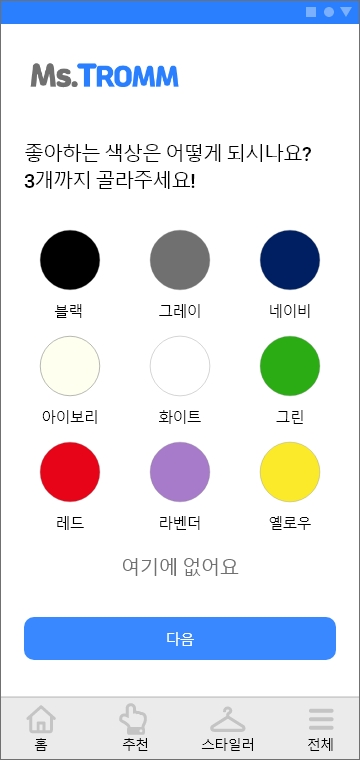
\includegraphics[scale=0.15]{설문지4.jpg}
                    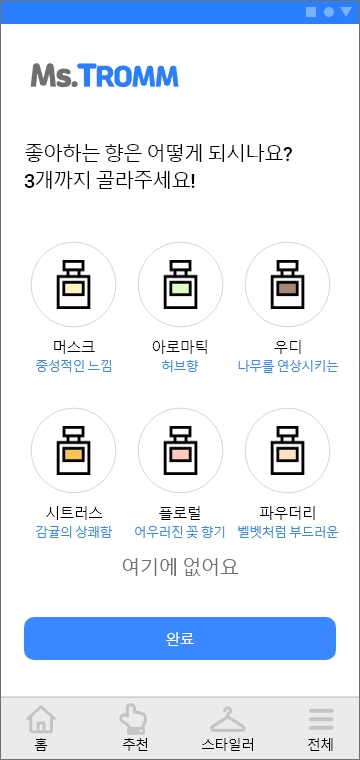
\includegraphics[scale=0.15]{설문지5.jpg}}
    \begin{itemize}
        \item[] \\ \\ This is a survey to increase the recommended accuracy of Ms. TROMM. The survey consists of questions about three elements (a style you usually wear often, a favorite color, and a favorite scent). In the case of frequently worn styles, different questions are provided depending on the gender entered when signing up as a member.\\
        \break
        \end{itemize} 
        \item Pop-up\\ \\
            \centerline{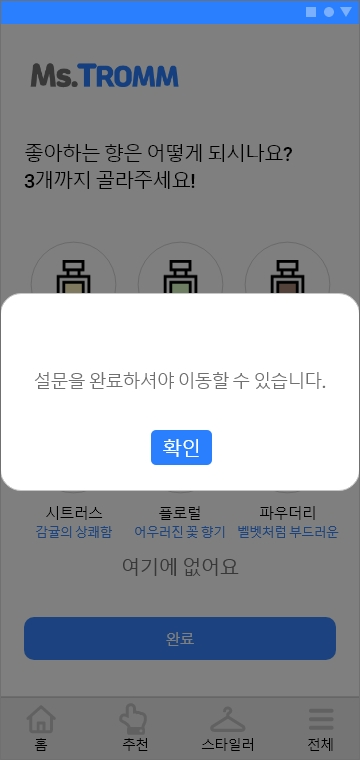
\includegraphics[scale=0.32]{설문지6.jpg}}
    \begin{itemize}
        \item[]  This is a pop-up that is exposed at the bottom of the questionnaire when you try to leave the page. "You must complete the survey to move!" will be displayed. When you click the gray area, 'x button', or 'OK button', the pop-up will end and the survey page will be exposed again.\\ \\ 
        \end{itemize} 

    \item Completed page \\ \\ \\
    \centerline{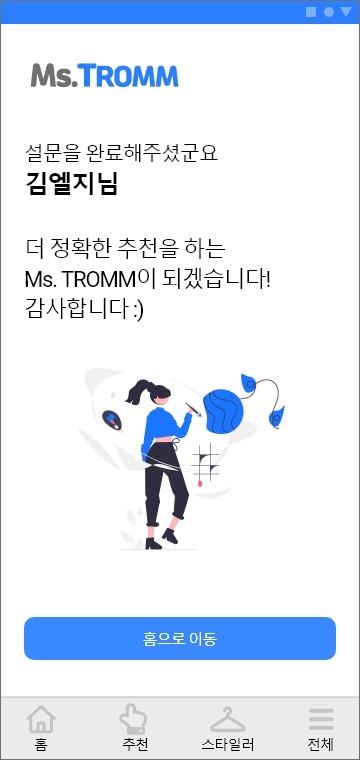
\includegraphics[scale=0.32]{설문지7.jpg}}
    \begin{itemize}
        \item[] This page appears when you complete the survey. The "Move to Home" button is exposed at the bottom. When clicking the button, go to Home.\\ \\ \\ \\
        \end{itemize} 
\end{enumerate}
\item Home(Main page)\\ \\
\centerline{\includegraphics[scale=0.32]{홈4.jpg}}
\begin{itemize}
    \item[] Home shows basic functions in the app at once.\\\\
\end{itemize}
 \begin{enumerate}
 \centerline{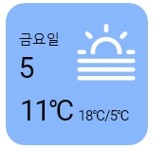
\includegraphics[scale=1]{일반 위젯.jpg}}
 \item[-]Indicate today's date and current weather. \\\\
 \leftline{
\includegraphics[scale=1]{오늘의 추천 위젯.jpg}}
 \item[-] Today's recommendation item is provided in the form of a preview of the recommendation that the user has set as the default recommendation.\\\\
 \item[-] Styler control items allow you to check the connection and connection status with the Styler/Smart Mirror and support the pause/react button when the Styler is operated. It also displays the remaining time until the styler operation stage and shutdown.\\\\
 \leftline{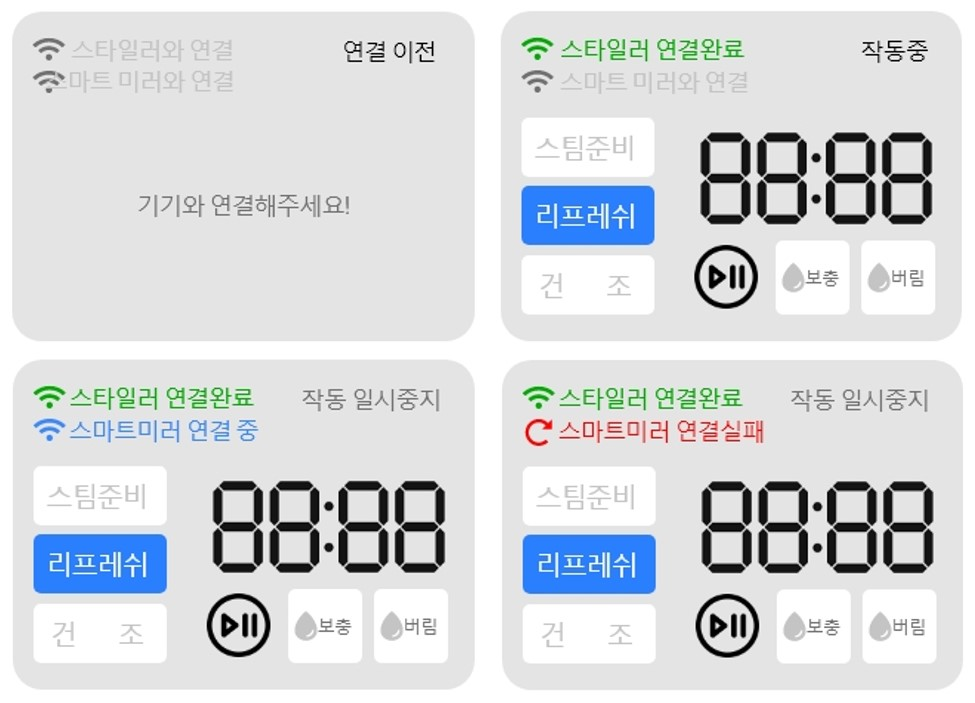
\includegraphics[scale=0.40]{스타일러 제어 위젯.jpg}}
 \break
 \item[-] \\ \\ If the styler/smart mirror is not connected, when clicked, it will be changed to a message indicating that the connection is underway and the color will be changed.\\\\
 \item[-] If the connection to the styler/smart mirror fails, it will be changed to a comment indicating the connection failure and the color will be changed.
 \leftline{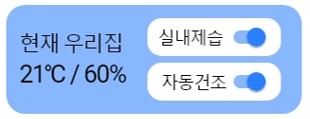
\includegraphics[scale=0.75]{현재 우리집 위젯.jpg}}
 \item[-] Current status of our home menu displays the temperature and humidity of the house, and buttons are located to turn on indoor dehumidification and automatic drying functions.\\
 \end{enumerate}
 \item Bottom Nav \\ \\ \\ \\
 \centerline{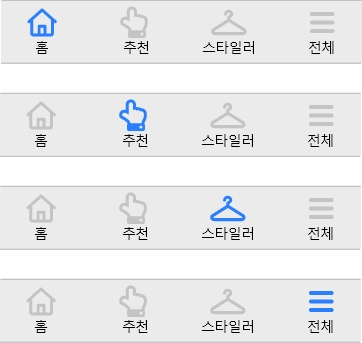
\includegraphics[scale=0.5]{하단 nav.jpg}}
 \break
 \begin{itemize}
    \item[] This is the bottom nav in the app. It consists of home, recommendation, styler, and whole, and when clicked, the picture is activated and goes to the page.
\end{itemize}
\end{enumerate}

\subsection{Pop-up} \\ \\
\begin{itemize}
    \item[] Notifications occurring in the app occur as pop-ups and can be found in the notification menu. You can enter the notification menu at the top of the home screen.\\ \\ \\
\end{itemize}
\begin{enumerate}
    \item Today's recommendation notification \\ \\
    \centerline{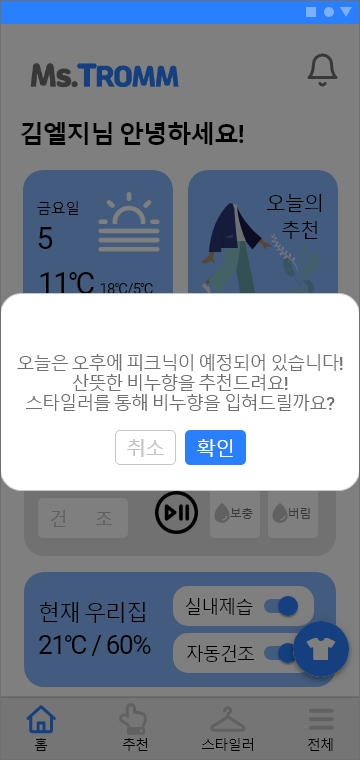
\includegraphics[scale=0.18]{오늘의 추천 팝업1.jpg}
    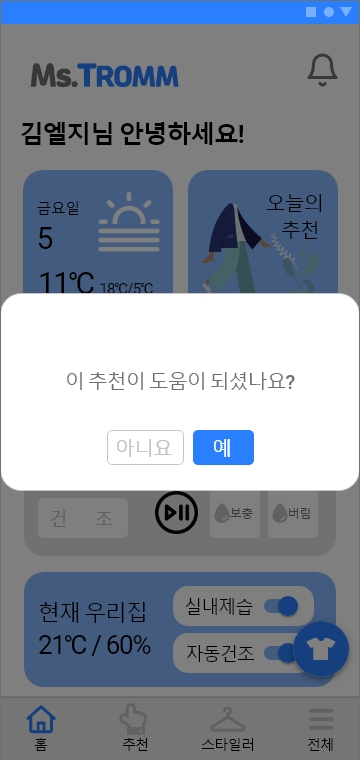
\includegraphics[scale=0.18]{오늘의 추천 팝업2.jpg}
    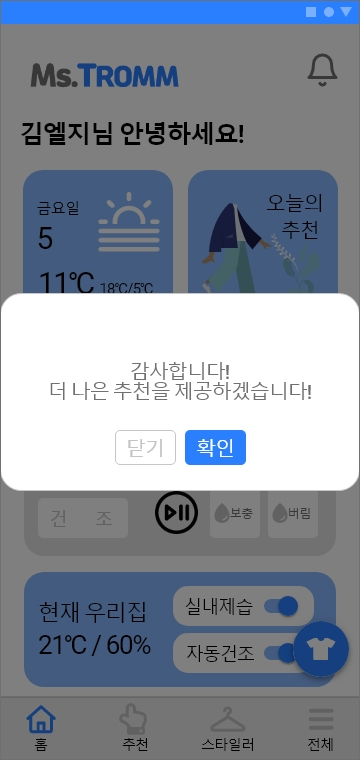
\includegraphics[scale=0.18]{오늘의 추천 팝업3.jpg}}
    \begin{itemize}
    \item[] Today's recommendation is caused by a pop-up notification. After checking the notification, a notification occurs to select whether the recommendation was helpful, and the recommendation termination popup is exposed when responding. Data from the notification asking for recommendation help is recorded on the server, and more personalized recommendations are made using it.\\
\end{itemize}
\item Control recommendation notification \\ \\ \\
\centerline{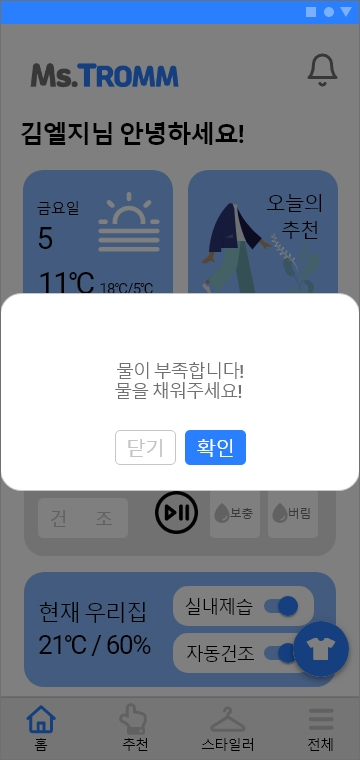
\includegraphics[scale=0.18]{제어추천 팝업1.jpg}
            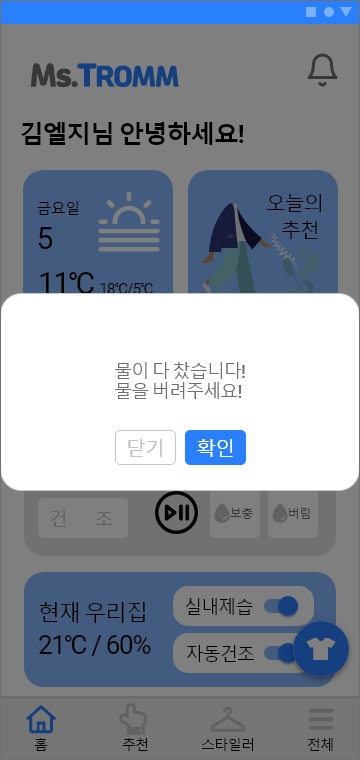
\includegraphics[scale=0.18]{제어추천 팝업2.jpg}}
\break
    \begin{itemize}
    \item[] This is a notification that occurs when there is a lack of water in the styler or when water needs to be discarded. \\ \\
\end{itemize}
\centerline{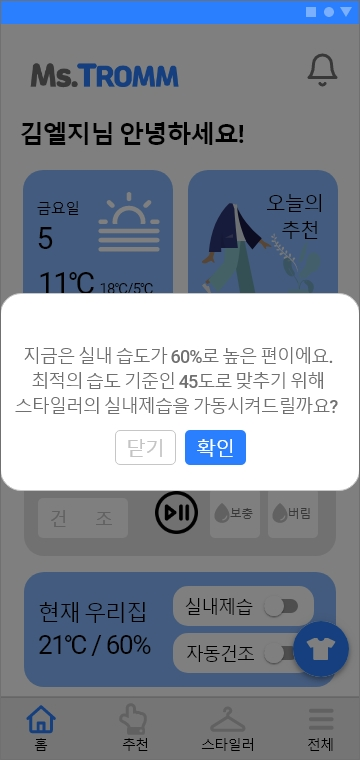
\includegraphics[scale=0.18]{제어추천 팝업3.jpg}
            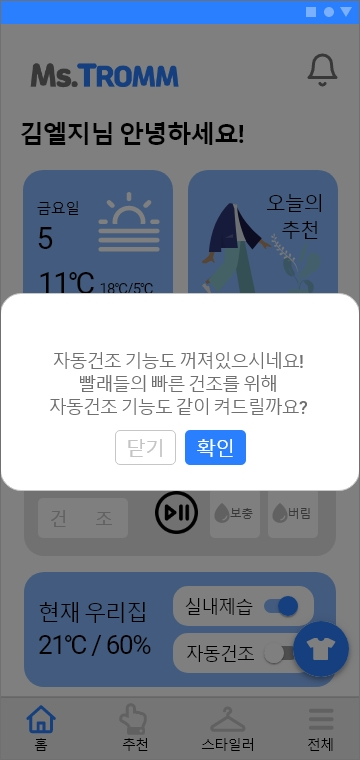
\includegraphics[scale=0.18]{제어추천 팝업4.jpg}}
\break
    \begin{itemize}
    \item[] This is a notification of indoor dehumidification and automatic drying control that occur when indoor humidity exceeds 40. \\ \\
\end{itemize}
     \item Weather notification\\ \\
     \centerline{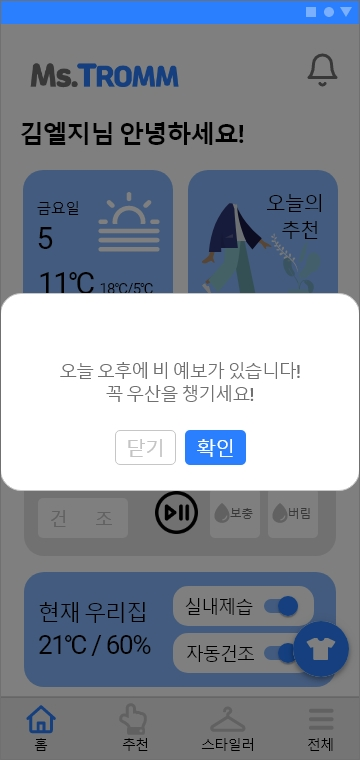
\includegraphics[scale=0.30]{날씨 추천 팝업.jpg}}
    \begin{itemize}
    \item[] \\ \\ \\ \\A pop-up notification occurs based on the weather. For example, if there's a rain forecast, you'll be notified to bring an umbrella..\\
\end{itemize}
     \item Schedule notification \\ \\
     \centerline{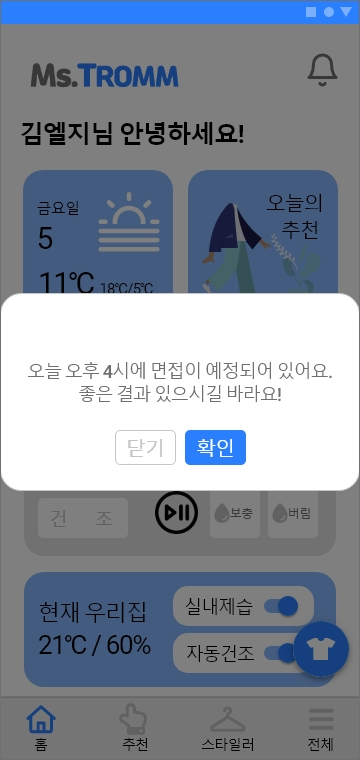
\includegraphics[scale=0.30]{일정 추천 팝업.jpg}}
    \begin{itemize}
    \item[] \\ \\ \\ \\ A pop-up notification occurs based on the schedule. For example, if you have an interview, you will be notified of the interview cheering comment\\
\end{itemize}
\end{enumerate}

\subsection{Notification} \\ \\
\begin{itemize}
    \item[] This is a menu in which the pop-up notification list that has occurred is recorded.\\ \\ \\
\end{itemize}
\begin{enumerate}
 \centerline{\includegraphics[scale=0.32]{알림1.jpg}}
 \item[-]\\This is the initial notification screen. Comments related to push alarm setting appear. \\\\\\\\
 \centerline{\includegraphics[scale=0.32]{알림2.jpg}}
 \item[-] This is a screen that is exposed when there is no notification history after replacing the push alarm setting to ON.\\\\\\\\
 \centerline{\includegraphics[scale=0.32]{알림3.jpg}}
 \item[-] \\\\ This is a screen that is exposed when there is a notification list.\\\\\\\\\\\\
\centerline{\includegraphics[scale=0.25]{알림4.jpg}
            \includegraphics[scale=0.25]{알림5.jpg}}
 \item[-] \\When you click on the notification list, the body containing the notification is exposed.\\\\\\\\\\\
 \end{enumerate}

\subsection{Recommendation}
\begin{itemize}
\item[] It's a menu that shows the recommendations. There are a total of two recommended criteria, including today's schedule and control. You can select the recommendation criteria at the top, and if you click the recommendation part of the recommendation, a pop-up related to fragrance use will occur.\\
\end{itemize}
    \begin{enumerate}
    \item Button description(first time to entry) \\ \\
    \centerline{\includegraphics[scale=0.32]{추천1.jpg}}
        \begin{itemize}
    \item[] When entering the recommendation menu for the first time, a page informing you of the basic functions of the buttons in the recommendation menu is exposed. It ends when you click on the gray area. \\
\end{itemize}
     \item Today's Recommendation \\ \\
     \centerline{\includegraphics[scale=0.32]{추천2.jpg}}
    \begin{itemize}
    \item[] \\ \\ \\ \\ This menu exposes today's recommendations using calendars and weather APIs. Comments and recommendations suitable for the date will be exposed.\\
\end{itemize}
       \item Control Recommendation \\ \\ \\
       \centerline{\includegraphics[scale=0.32]{추천3.jpg}}
       \break
           \begin{itemize}
    \item[] It is a menu that provides recommendations related to the clothing and home environment in the styler.\\\\\\
\end{itemize}
     \item Pop-up related to fragrance use \\ \\
     \centerline{\includegraphics[scale=0.25]{추천4.jpg}
                \includegraphics[scale=0.25]{추천5.jpg}}
    \begin{itemize}
    \item[] \\ \\ \\ \\ This is a pop-up that is exposed when you click the fragrance recommendation part. Ask questions about applying the Styler Introductory Application, and forward the sheet activation command to the Styler when the user wants to apply the fragrance.\\
\end{itemize}
\end{enumerate}

\subsection{Styler}  \\ 
\centerline{\includegraphics[scale=0.32]{스타일러4.jpg}}
This is a menu where you can control the styler. Control buttons on the styler are exposed.
 \begin{enumerate}
\centerline{\includegraphics[scale=0.32]{스타일러1.jpg}}
 \item[-]This is a page that appears when not connected to the styler. \\\\
\centerline{\includegraphics[scale=0.5]{제어 버튼1.jpg}} \\ \\
\centerline{\includegraphics[scale=0.5]{제어 버튼2.jpg}} \\ \\
\centerline{\includegraphics[scale=0.5]{제어 버튼3.jpg}} \\ \\
 \item[-]It's related to the operation of the styler. There are Styler power-on, power-off, start operation, stop operation buttons, and reservation buttons. If the styler is running, it displays which function is running. \\\\
  \centerline{\includegraphics[scale=0.5]{스타일러 버튼.jpg}}
 \item[-]It's a menu that can be operated by the styler. It supports a total of six functional operations \\\\
\centerline{\includegraphics[scale=0.3]{스타일링 선택.jpg}
            \includegraphics[scale=0.3]{섬세건조 선택.jpg}} \\ \\
\centerline{\includegraphics[scale=0.3]{고급의류 선택.jpg}
            \includegraphics[scale=0.3]{스팀살균 선택.jpg}} \\ \\
 \item[-]Details of the course will be exposed when each button is clicked. \\\\
   \centerline{\includegraphics[scale=0.32]{스타일러7.jpg}}
 \item[-]This is a pop-up that is exposed when another styler menu is pressed while the styler is running. \\\\
 \end{enumerate}
 
\subsection{My Closet}  \\
The button to enter my closet menu continues to be exposed to a floating action button within the app.
\begin{enumerate}
\item My Closet\\ \\
 \begin{enumerate}
 \centerline{\includegraphics[scale=0.32]{내 옷장1.jpg}}
 \item[-]The registration date of the clothes and the date you put them in the styler most recently are displayed. The clothes bookmarked at the top are currently in the styler. \\\\
 \item[-]Clothes that need to be turned around in the styler will be guided above. We need a styler in order of importance. - How about a styler?This outfit is okay. \\\\
 \centerline{\includegraphics[scale=0.32]{내 옷장2.jpg}}
 \item[-] When you click on the bottom of the list, detailed information about the clothes appears. The information that appears is the registration date, the last styler working day, and the contents that were registered when registering clothes.\\\\
 \end{enumerate}
 
 \item Register New clothes\\ \\
 \begin{enumerate}
    \centerline{\includegraphics[scale=0.24]{새 옷 등록하기1.jpg}
    \includegraphics[scale=0.24]{새 옷 등록하기2.jpg}}
 \item[-]It's a menu to register new clothes. At first, the part where you put the picture of the clothes and the name input field are exposed. \\\\
 \centerline{\includegraphics[scale=0.32]{새 옷 등록하기3.jpg}}
 \item[-]Next, fields where you can enter colors, styling courses, high-end drying courses, and sterilization are exposed. \\\\
  \centerline{\includegraphics[scale=0.32]{새 옷 등록하기4.jpg}}
 \item[-]This is a screen where a guide phrase for designating no category is exposed as a pop-up. \\\\
  \centerline{\includegraphics[scale=0.32]{새 옷 등록하기5.jpg}}
 \item[-]This is a pop-up announcing the completion of the procedure for registering new clothes. \\\\
 \end{enumerate}
 \end{enumerate}

\subsection {All} \\
This is a menu where you can check the general information of the app. You can check the subscription information and version information terms and conditions, and there is a menu that allows you to change the default settings in the app.
\begin{enumerate}
    \item Login form screen \\ \\
    \centerline{\includegraphics[scale=0.32]{전체.jpg}}
    \begin{itemize}
    \item[] Version information is displayed in this menu page. \\
    \end{itemize}
    \item My information \\\\
    \centerline{\includegraphics[scale=0.32]{내 정보1.jpg}}
    \begin{itemize}
    \item[] This is a menu where you can check the information you entered when signing up. If you want to change the information, click the Change button at the bottom to see the Change screen. \\ \\
    \end{itemize}
    \centerline{\includegraphics[scale=0.32]{내 정보2.jpg}}
    \begin{itemize}
    \item[] After pressing Change, the screen is displayed. You can modify the information you entered when signing up. \\ \\
    \end{itemize}
    \item Terms and Conditions \\ \\ \\
    \centerline{\includegraphics[scale=0.32]{개인정보약관.jpg}}
    \begin{itemize}
    \item[]You can check the terms and conditions of using personal information. \\ \\ \\ \\ \\ \\ \\ \\ \\ \\ \\ \\ \\ \\
    \end{itemize}
\end{enumerate}



% \subsection{Equations}
% Number equations consecutively. To make your 
% equations more compact, you may use the solidus (~/~), the exp function, or 
% appropriate exponents. Italicize Roman symbols for quantities and variables, 
% but not Greek symbols. Use a long dash rather than a hyphen for a minus 
% sign. Punctuate equations with commas or periods when they are part of a 
% sentence, as in:
% \begin{equation}
% a+b=\gamma\label{eq}
% \end{equation}

% Be sure that the 
% symbols in your equation have been defined before or immediately following 
% the equation. Use ``\eqref{eq}'', not ``Eq.~\eqref{eq}'' or ``equation \eqref{eq}'', except at 
% the beginning of a sentence: ``Equation \eqref{eq} is . . .''

% \subsection{\LaTeX-Specific Advice}

% Please use ``soft'' (e.g., \verb|\eqref{Eq}|) cross references instead
% of ``hard'' references (e.g., \verb|(1)|). That will make it possible
% to combine sections, add equations, or change the order of figures or
% citations without having to go through the file line by line.

% Please don't use the \verb|{eqnarray}| equation environment. Use
% \verb|{align}| or \verb|{IEEEeqnarray}| instead. The \verb|{eqnarray}|
% environment leaves unsightly spaces around relation symbols.

% Please note that the \verb|{subequations}| environment in {\LaTeX}
% will increment the main equation counter even when there are no
% equation numbers displayed. If you forget that, you might write an
% article in which the equation numbers skip from (17) to (20), causing
% the copy editors to wonder if you've discovered a new method of
% counting.

% {\BibTeX} does not work by magic. It doesn't get the bibliographic
% data from thin air but from .bib files. If you use {\BibTeX} to produce a
% bibliography you must send the .bib files. 

% {\LaTeX} can't read your mind. If you assign the same label to a
% subsubsection and a table, you might find that Table I has been cross
% referenced as Table IV-B3. 

% {\LaTeX} does not have precognitive abilities. If you put a
% \verb|\label| command before the command that updates the counter it's
% supposed to be using, the label will pick up the last counter to be
% cross referenced instead. In particular, a \verb|\label| command
% should not go before the caption of a figure or a table.

% Do not use \verb|\nonumber| inside the \verb|{array}| environment. It
% will not stop equation numbers inside \verb|{array}| (there won't be
% any anyway) and it might stop a wanted equation number in the
% surrounding equation.

% \subsection{Some Common Mistakes}\label{SCM}
% \begin{itemize}
% \item The word ``data'' is plural, not singular.
% \item The subscript for the permeability of vacuum $\mu_{0}$, and other common scientific constants, is zero with subscript formatting, not a lowercase letter ``o''.
% \item In American English, commas, semicolons, periods, question and exclamation marks are located within quotation marks only when a complete thought or name is cited, such as a title or full quotation. When quotation marks are used, instead of a bold or italic typeface, to highlight a word or phrase, punctuation should appear outside of the quotation marks. A parenthetical phrase or statement at the end of a sentence is punctuated outside of the closing parenthesis (like this). (A parenthetical sentence is punctuated within the parentheses.)
% \item A graph within a graph is an ``inset'', not an ``insert''. The word alternatively is preferred to the word ``alternately'' (unless you really mean something that alternates).
% \item Do not use the word ``essentially'' to mean ``approximately'' or ``effectively''.
% \item In your paper title, if the words ``that uses'' can accurately replace the word ``using'', capitalize the ``u''; if not, keep using lower-cased.
% \item Be aware of the different meanings of the homophones ``affect'' and ``effect'', ``complement'' and ``compliment'', ``discreet'' and ``discrete'', ``principal'' and ``principle''.
% \item Do not confuse ``imply'' and ``infer''.
% \item The prefix ``non'' is not a word; it should be joined to the word it modifies, usually without a hyphen.
% \item There is no period after the ``et'' in the Latin abbreviation ``et al.''.
% \item The abbreviation ``i.e.'' means ``that is'', and the abbreviation ``e.g.'' means ``for example''.
% \end{itemize}
% An excellent style manual for science writers is \cite{b7}.

% \subsection{Authors and Affiliations}
% \textbf{The class file is designed for, but not limited to, six authors.} A 
% minimum of one author is required for all conference articles. Author names 
% should be listed starting from left to right and then moving down to the 
% next line. This is the author sequence that will be used in future citations 
% and by indexing services. Names should not be listed in columns nor group by 
% affiliation. Please keep your affiliations as succinct as possible (for 
% example, do not differentiate among departments of the same organization).

% \subsection{Identify the Headings}
% Headings, or heads, are organizational devices that guide the reader through 
% your paper. There are two types: component heads and text heads.

% Component heads identify the different components of your paper and are not 
% topically subordinate to each other. Examples include Acknowledgments and 
% References and, for these, the correct style to use is ``Heading 5''. Use 
% ``figure caption'' for your Figure captions, and ``table head'' for your 
% table title. Run-in heads, such as ``Abstract'', will require you to apply a 
% style (in this case, italic) in addition to the style provided by the drop 
% down menu to differentiate the head from the text.

% Text heads organize the topics on a relational, hierarchical basis. For 
% example, the paper title is the primary text head because all subsequent 
% material relates and elaborates on this one topic. If there are two or more 
% sub-topics, the next level head (uppercase Roman numerals) should be used 
% and, conversely, if there are not at least two sub-topics, then no subheads 
% should be introduced.

% \subsection{Figures and Tables}
% \paragraph{Positioning Figures and Tables} Place figures and tables at the top and 
% bottom of columns. Avoid placing them in the middle of columns. Large 
% figures and tables may span across both columns. Figure captions should be 
% below the figures; table heads should appear above the tables. Insert 
% figures and tables after they are cited in the text. Use the abbreviation 
% ``Fig.~\ref{fig}'', even at the beginning of a sentence.

% \begin{table}[htbp]
% \caption{Table Type Styles}
% \begin{center}
% \begin{tabular}{|c|c|c|c|}
% \hline
% \textbf{Table}&\multicolumn{3}{|c|}{\textbf{Table Column Head}} \\
% \cline{2-4} 
% \textbf{Head} & \textbf{\textit{Table column subhead}}& \textbf{\textit{Subhead}}& \textbf{\textit{Subhead}} \\
% \hline
% copy& More table copy$^{\mathrm{a}}$& &  \\
% \hline
% \multicolumn{4}{l}{$^{\mathrm{a}}$Sample of a Table footnote.}
% \end{tabular}
% \label{tab1}
% \end{center}
% \end{table}

% \begin{figure}[htbp]
% \centerline{\includegraphics{fig1.png}}
% \caption{Example of a figure caption.}
% \label{fig}
% \end{figure}

% Figure Labels: Use 8 point Times New Roman for Figure labels. Use words 
% rather than symbols or abbreviations when writing Figure axis labels to 
% avoid confusing the reader. As an example, write the quantity 
% ``Magnetization'', or ``Magnetization, M'', not just ``M''. If including 
% units in the label, present them within parentheses. Do not label axes only 
% with units. In the example, write ``Magnetization (A/m)'' or ``Magnetization 
% \{A[m(1)]\}'', not just ``A/m''. Do not label axes with a ratio of 
% quantities and units. For example, write ``Temperature (K)'', not 
% ``Temperature/K''.

% \section*{Acknowledgment}

% The preferred spelling of the word ``acknowledgment'' in America is without 
% an ``e'' after the ``g''. Avoid the stilted expression ``one of us (R. B. 
% G.) thanks $\ldots$''. Instead, try ``R. B. G. thanks$\ldots$''. Put sponsor 
% acknowledgments in the unnumbered footnote on the first page.

% \section*{References}

% Please number citations consecutively within brackets \cite{b1}. The 
% sentence punctuation follows the bracket \cite{b2}. Refer simply to the reference 
% number, as in \cite{b3}---do not use ``Ref. \cite{b3}'' or ``reference \cite{b3}'' except at 
% the beginning of a sentence: ``Reference \cite{b3} was the first $\ldots$''

% Number footnotes separately in superscripts. Place the actual footnote at 
% the bottom of the column in which it was cited. Do not put footnotes in the 
% abstract or reference list. Use letters for table footnotes.

% Unless there are six authors or more give all authors' names; do not use 
% ``et al.''. Papers that have not been published, even if they have been 
% submitted for publication, should be cited as ``unpublished'' \cite{b4}. Papers 
% that have been accepted for publication should be cited as ``in press'' \cite{b5}. 
% Capitalize only the first word in a paper title, except for proper nouns and 
% element symbols.

% For papers published in translation journals, please give the English 
% citation first, followed by the original foreign-language citation \cite{b6}.

% \begin{thebibliography}{00}
% \bibitem{b1} G. Eason, B. Noble, and I. N. Sneddon, ``On certain integrals of Lipschitz-Hankel type involving products of Bessel functions,'' Phil. Trans. Roy. Soc. London, vol. A247, pp. 529--551, April 1955.
% \bibitem{b2} J. Clerk Maxwell, A Treatise on Electricity and Magnetism, 3rd ed., vol. 2. Oxford: Clarendon, 1892, pp.68--73.
% \bibitem{b3} I. S. Jacobs and C. P. Bean, ``Fine particles, thin films and exchange anisotropy,'' in Magnetism, vol. III, G. T. Rado and H. Suhl, Eds. New York: Academic, 1963, pp. 271--350.
% \bibitem{b4} K. Elissa, ``Title of paper if known,'' unpublished.
% \bibitem{b5} R. Nicole, ``Title of paper with only first word capitalized,'' J. Name Stand. Abbrev., in press.
% \bibitem{b6} Y. Yorozu, M. Hirano, K. Oka, and Y. Tagawa, ``Electron spectroscopy studies on magneto-optical media and plastic substrate interface,'' IEEE Transl. J. Magn. Japan, vol. 2, pp. 740--741, August 1987 [Digests 9th Annual Conf. Magnetics Japan, p. 301, 1982].
% \bibitem{b7} M. Young, The Technical Writer's Handbook. Mill Valley, CA: University Science, 1989.
% \end{thebibliography}
% \vspace{12pt}
% \color{red}
% IEEE conference templates contain guidance text for composing and formatting conference papers. Please ensure that all template text is removed from your conference paper prior to submission to the conference. Failure to remove the template text from your paper may result in your paper not being published.

\end{document}
